\documentclass{beamer}
\usepackage{amsmath,amssymb,amsthm,array}
\usepackage{xltxtra}
\usepackage{multirow}
\usepackage{multicol}
\usepackage{algorithm}
\usepackage{algorithmic}
\usetheme{CambridgeUS}
\usecolortheme{seagull}
\usefonttheme{serif}
\setbeamertemplate{navigation symbols}{}
\title{Voting with Mixnets}
\author{Panagiotis Grontas}
\date{1/2/2013 - 15/2/2013}
\defbeamertemplate*{footline}{shadow theme}
{%
  \leavevmode%
  \hbox{\begin{beamercolorbox}[wd=.5\paperwidth,ht=2.5ex,dp=1.125ex,leftskip=.3cm plus1fil,rightskip=.3cm]{author in head/foot}%
    \usebeamerfont{author in head/foot}\insertframenumber\,/\,\inserttotalframenumber\hfill\insertshortauthor (\insertshortinstitute)
  \end{beamercolorbox}%
  \begin{beamercolorbox}[wd=.5\paperwidth,ht=2.5ex,dp=1.125ex,leftskip=.3cm,rightskip=.3cm plus1fil]{title in head/foot}%
    \usebeamerfont{title in head/foot}\insertshorttitle%
  \end{beamercolorbox}}%
  \vskip0pt%
}
\institute{$\mu\Pi\lambda\forall$  - CoReLab Crypto Group}

\setlength{\columnseprule}{0.4pt}
\begin{document}

\begin{frame}
\titlepage
\end{frame}

\begin{frame}{Outline}
\begin{itemize}
\item Election System Abstraction And Properties
\item Crypto Preliminaries
\item Mixnets: Definition And Types
\item Zero Knowledge Verifiable Mixnets
\item Other Types of Verifiable Mixnets
\end{itemize}
\end{frame}

\section{Election System Abstraction And Properties}

\begin{frame}{High Level properties \cite{JAH12}}
\begin{itemize}
\item \textbf{Integrity}
\begin{itemize}
	\item Votes are cast as intended
	\item Votes are counted as cast
\end{itemize}
\item \textbf{Ballot Secrecy} Nobody can figure out how you voted (privacy), even if you try to prove it (selling/coercion).
\item Authentication and Authorisation
\begin{itemize}
	\item Only authorised voters can vote
	\item a specified number of times as stated in election law
\end{itemize}
\item Enfranchisement All voters must have the opportunity to vote
\item Availability (DoS,Tallying)
\item Efficiency (Cost,Time)
\end{itemize}
\textbf{Remark:} Authentication vs Secrecy vs Enfranchisement
\end{frame}
 

\begin{frame}{Low Level Properties \cite{Riv6897}}
\begin{itemize}
\item \textbf{Individual Verifiability} Each voter can check that their ballot was included in the outcome
\item \textbf{Universal Verifiability} All voters can check that a voter's ballot was included in the outcome
\item \textbf{Receipt - Freeness} A voter cannot prove how she voted even if she wants to.
\item \textbf{Robust} Nobody can disrupt an election
\item \textbf{Fairness} No partial results are known.
\item \textbf{Eliminate Vote Duplication} A voter can figure another vote by duplicating it and checking the bulletin board for a correlated vote.
\item \textbf{Vote Cancelling} Vote in such way as to nullify a vote (without knowing it)
\end{itemize}
\textbf{Remark:}Individual Verifiability vs Receipt - Freeness
\end{frame}

\section{Crypto Preliminaries}

\begin{frame}{ElGamal Encryption}
\begin{itemize}
\item Randomised Public Key Encryption From Diffie Hellman 
\item KeyGen From Cyclic Group $<g>$ of prime order $q$
\begin{itemize}
\item  $ x \in_R \mathbb{Z}_q $
\item  $ y = g^x mod p $
\item  return $ (pk = <<p,q,g>,y>, sk = x)$
\end{itemize}
\item Encrypt Message $m$ with public key $y$
\begin{itemize}
\item  encode $m \in <g>$
\item  $r \in_R \mathbb{Z}_q$
\item  $G = g^r \, mod p$
\item  $M = m \cdot y^r \, mod p$
\item  return $(G,M)$
\end{itemize}
\item Decrypt message $(G,M)$ with secret key $x$
\begin{itemize}
\item  return $M/G^x \, mod p$
\end{itemize}
\end{itemize}
\end{frame}

\begin{frame}{ElGamal Re Encryption - Re Randomisation \cite{AdidaGoogle}}
\begin{align*}
 ReEnc(c,r') & = c \cdot Enc(1,r') \\
	 & = (g^r, m \cdot (g^x)^{r}) \cdot (g^{r'}, (g^x)^{r'}) \\
	 & = (g^{r+r'},m \cdot (g^x)^{r+r'}) 
\end{align*}
\begin{itemize}
\item No knowledge of secret key is required.
\item Re encryption does not affect decryption
\item Without the secret key or the re randomisation factor it is infeasible to show that two messages are re reencryptions of each other (subject to the DDH)
\end{itemize}
\end{frame}

\begin{frame}{ElGamal Multiplicative Homomorphism}
\begin{itemize}
\item Let $m_1, m_2$ plaintexts. Then:
$Enc(m_1) \cdot Enc(m_2) = Enc(m_1 \cdot m_2)$
\item 
\begin{align*}
 Enc(m_1) \cdot Enc(m_2) = \\
 ( g^{r_1},m_1 \cdot y^{r_1} ) \cdot ( g^{r_2},m_2 \cdot y^{r_2} ) = \\
 ( g^{r_1+r_2},m_1 \cdot m_2 y^{r_1+r_2} ) = \\
 Enc(m_1 \cdot m_2)
\end{align*}
\item In elections we would desire additive homomorphism.
\end{itemize}
\end{frame}

\begin{frame}{Prove that you know DLOG (Schnorr)}
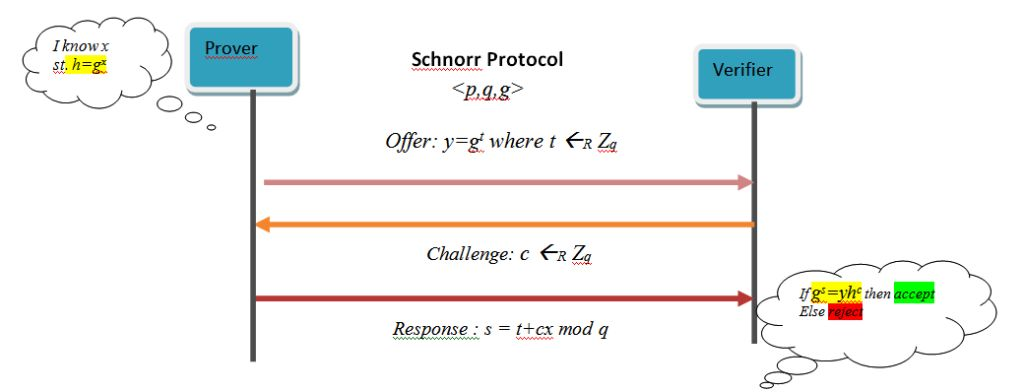
\includegraphics[scale=0.4]{schnorr.jpg}
\begin{itemize}
\item Non interactive version (Fiat-Shamir)
\item Replace challenge with hash $ H(g^t) $ 
\end{itemize}
\end{frame} 

\begin{frame}{Prove DLOG equality (Chaum-Pedersen)}
\begin{center}
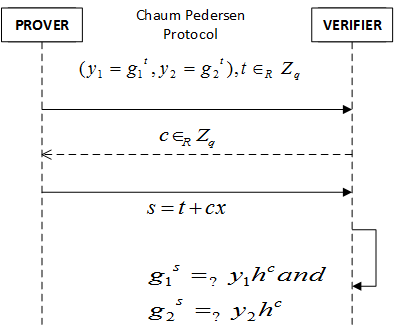
\includegraphics[scale=0.3]{chaumpedersen.jpg}
\end{center}
\begin{itemize}
\item  Honest-Verifier Zero Knowledge
\end{itemize}
\end{frame} 

\section{Mixnets - Definition And Problems}

\begin{frame}{Mixnet Overview}
\begin{itemize}
\item Introduced in \cite{Chaum81}
\item Primitive for anonymous channel
\item Many uses: elections (of course), anonymous browsing etc.
\item Operation: Different mistrusting parties
\item Anonymity based on encryption+shuffling
\item Output a random permutation of the input
\item No single output item, must match an input item
\item Enter encryption
\end{itemize}
\begin{center}

\includegraphics[scale=0.3]{shuffle2.jpg}
\end{center}
\end{frame} 

\begin{frame}{Mixnets}
\begin{center}
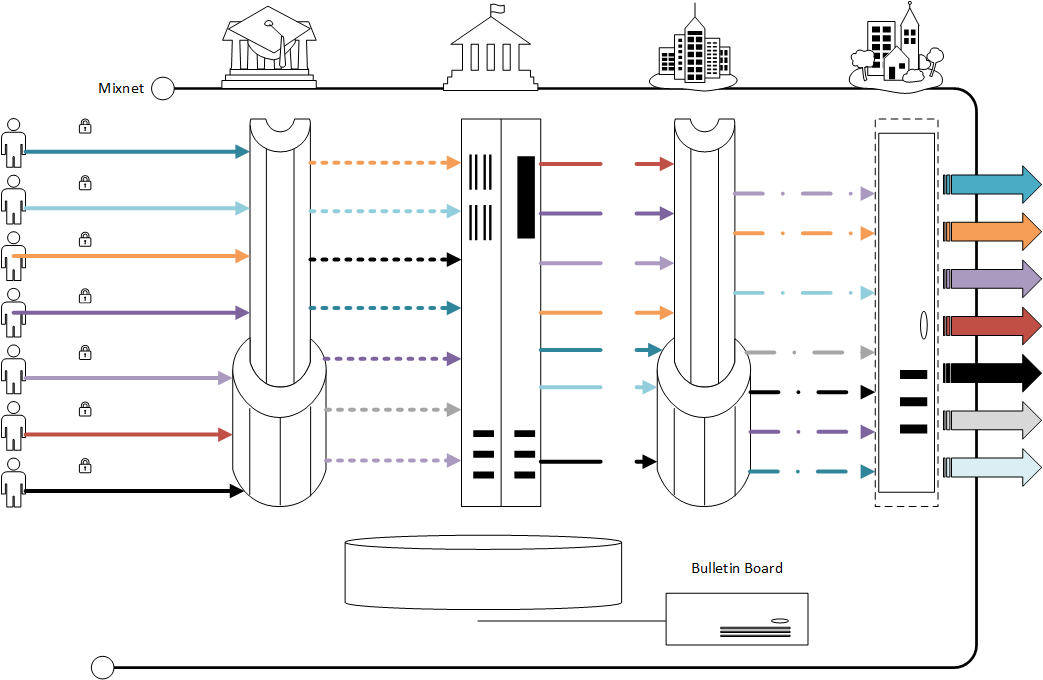
\includegraphics[scale=0.4]{mix.jpg}
\end{center}
\end{frame} 

\begin{frame}{Bulletin Board}
\begin{itemize}
\item Essential Component of All Election Systems
\item Integrity Preserving Tallying: Post all votes, Public tallying
\item Authenticated
\item Accessible to the public
\item Tamper Proof
\item Resistant to DoS attacks
\item Each mix server reads input and appends output
\item Implemented via Byzantine agreement algorithms
\end{itemize}
\end{frame}

\begin{frame}{Voting With Mixnets:Main Idea}
\begin{itemize}
\item Create Ballots
\item Initial Encryption $C_{10},C_{20},....,C_{n0} = Enc(B_1,...,B_n)$
\item Each mix server processes and permutes the encrypted items
\item After all mixing has occured (optionally) decrypt items
\item Post the \textbf{unencrypted ballots} to the bulletin board
\item Perform the tally
\end{itemize}
\end{frame} 

\begin{frame}{Decryption Mixnets}
\begin{itemize}
\item The original \cite{Chaum81} idea
\item Encrypt the ballot with the public key of the mix servers in reverse order
\item $ C_{i0} = E_{pk1} \circ E_{pk2} \circ ... \circ E_{pkt} (B_i) $
\item Each mix server decrypts with its secret key (akin to onion peeling) and performs the shuffle
\item After the final stage, all ballots are decrypted
\item The final decryption key might shared.
\item \textbf{Remarks:} 
\begin{itemize}
\item A mix server can block the mixing process
\item The ciphertext size is proportional to the number of mix servers
\end{itemize} 
\end{itemize}
\end{frame} 

\begin{frame}{ReEncryption Mixnets \cite{PIK93}}

\begin{itemize} 
\item Two variations both of them proposed in \cite{PIK93}
\item Version 1
\begin{itemize}
	\item Each mix server re randomises the ballots by reencryption
	\item A final decryption stage is needed
	\item The decryption key must be shared to various parties
	\item The decryption is jointly done by all mix servers.
\end{itemize}
\item Version 2
\begin{itemize}
	\item Each mix server partially decrypts the ballots by applying its secret key.
	\item Then re randomises by reencryption
	\item The last mix server decrypts
\end{itemize}
\item Elgamal, Pallier Cryptosystems
\end{itemize}

\end{frame} 

\begin{frame}{Is everything OK?}
\begin{block}{Yes provided that:}
\begin{itemize}
\item We trust the original encryption
\item We trust at least one mix server
\item We trust the decryption (Honest Majority Needed)
\item We only want individual verifiability, but not universal.
\end{itemize}
\end{block}
\begin{block}{Universal Verifiability - Verification}
\begin{itemize}
\item for each decryption/reencryption
\item for the correct permutation
\end{itemize}
\textit{without compromising anonymity}
\end{block}

\end{frame} 

\begin{frame}{What can go wrong}
\begin{itemize}
\item At the initial encryption stage, a different vote might be encrypted (vote changing, vote copying, vote cancelling)
\item \textbf{Solution:Zero - knowledge proof of the contents of the vote}
\item A mix server can change some of the input votes, by replacing them in the output.
\item \textbf{Solution:Zero - knowledge proof of correct shuffling for the mix-servers}
\item A subset of the mix servers might cooperate to break anonymity
\item \textbf{Solution:Privacy is guaranteed if at least one of the mix servers is honest}
\end{itemize}
\end{frame} 

\section{Zero Knowledge Verifiable Mixnets}

\begin{frame}{General Idea}
\begin{itemize}
\item Correctness of initial encryption $ \Leftrightarrow $ Prove that you know DLOG
\small
\item Correctness of Shuffling\cite{Riv6897} $ \Leftrightarrow $ \\
	Prove that each encrypted vote in the input, appears in the output $ \Leftrightarrow $\\
	Prove that each encrypted vote in the input, has a reencryption in the output $ \Leftrightarrow $\\
	Prove the following NP statement 
\normalsize
\begin{align*}
\exists  \text{ permutation } \pi  \text { on }   \{1,\cdots, n \}, \exists  s_1,...,s_n, \\
\forall  \text{ vote }  i \in \{1,\cdots, n \}, \\
\forall   \text{ mix server }  j \in \{1, \cdots, k \}  :\\ 
\text{ If }  C_{i,j} = (a_{i,j},b_{i,j})  \text{ and }  C_{\pi(i),j+1} = (a_{\pi(i),j},b_{\pi(i),j})  \text{ then } \\
a_{\pi(i),j+1} = a_{i,j} \cdot g^{s_i} \text{ and }
b_{\pi(i),j+1} = b_{i,j} \cdot y^{s_i}
\end{align*}

\item NP-statement $\Rightarrow$ Zero-Knowledge Proof
\item How fast?
\end{itemize}
\end{frame}

\begin{frame}{An example:Millimix \cite{JJ99}}
\begin{itemize}
\item A mixnet with the following properties:
\begin{itemize}
\item Privacy: Correlation of input/output no better than a random guess
\item Robustness: The output of each mich server is a correct reencryption and permutation
\item Public Verifiability: Anybody (participant or not) can verify the correct operation
\item Computational Efficiency on small batches
\end{itemize}
\end{itemize}
\end{frame}

\begin{frame}[allowframebreaks]{Millimix Architecture}
\begin{block}{Sorting Networks}
\begin{itemize}
\item A collection of wires and comparators. 
\item A $2\times2$ comparator is a function $f$ such that:
\[
f(x,y) = \begin{cases} (x,y), & \text{ if }  x<y  \\ (y,x), & \text{ if } x \geq y  \end{cases}
\]
\item n input wires, n output wires that are connected by comparators
\item Result: Inputs are outputted in sorted order.
\item \textbf{Remark:} Can implement all $n!$ permutations.
\item At least $\Omega(nlogn)$ comparators. 
\end{itemize}
\end{block}
\begin{itemize}
\framebreak
\item Each mix server $S_i$ simulates a sorting network.
\item Generates a random permutation $\pi_i$
\item Output $E_u,E_v$ based on the comparison $\pi_1(u), \pi_1(v)$
\item The mix network as a whole simulates the permutation: $\pi = \pi_n \circ \cdots \circ \pi_1$
\end{itemize}
\end{frame}

\begin{frame}{Millimix:Proof Of Reencryption}
\begin{block}{Statement}
The ciphertext $c_2 = (a_2,b_2) = (g_u,m_2 \cdot y_u)$ is a reencryption of the ciphertext $c_1 = (a_1,b_1) = (g_t,m_1 \cdot y_t)$
\end{block}
\begin{block}{Proof}
$c_2$ is a reencryption of $c_1$ iff they both encrypt the same message, meaning that $m_1=m_2$.
\begin{align*}
m_1 = m_2 \Leftrightarrow  \frac{m_1}{m_2} = 1 \Leftrightarrow  \frac{m_1 \cdot y^t}{m_2 \cdot y^u} = \frac{y^t}{y^u} \Leftrightarrow\\  \frac{b_1}{b_2} = \frac{a_{1}^{x}}{a_{2}^{x}} \Leftrightarrow log_{a_1}b_1 = x  \text{  and  } log_{a_2}b_2 = x \Leftrightarrow\\   log_{a_1}b_1 = log_{a_2}b_2 \Leftrightarrow  \text{ Chaum - Pedersen Protocol }
\end{align*}
\end{block}
\end{frame}

\begin{frame}[allowframebreaks]{Millimix:Proof Of Permutation}

\begin{block}{Statement}
Prove that $\{c'_1,\cdots,c'_n\}$ is a reencryption of $\{c_1,\cdots,c_n\}$ without revealing the correspondence.
\end{block}

\begin{block}{Proof}
Denote $c_1 \approx c_2$ iff $c_1$ is a reencryption of $c_2$.
We shall first prove for a $2\times2$ mix server that
$(c'_1 \approx c_1 \bigwedge c'_2 \approx c_2) \bigvee (c'_1 \approx c_2 \bigwedge c'_2 \approx c_1)$
\begin{center}
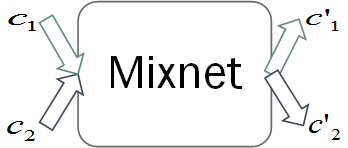
\includegraphics[scale=0.25]{mix2x2.jpg}
\end{center}
\begin{scriptsize}
$\Leftrightarrow (c'_1 \approx c_1 \vee c'_1 \approx c_2) 
  \bigwedge 
 (c'_1 \approx c_1 \vee c'_2 \approx c_1)
  \bigwedge  
 (c'_2 \approx c_2 \vee c'_1 \approx c_2) 
  \bigwedge 
 (c'_2 \approx c_2 \vee c'_2 \approx c_1)  
$
\end{scriptsize}
\end{block}

\begin{block}{Prove  $(c'_1 \approx c_1 \vee c'_1 \approx c_2)$}
Use the Chaum-Pedersen Protocol and accept if $c'_1 \approx c_1$ or $c'_2 \approx c_2$.
\end{block}
\begin{itemize}
\item Generalize for $n \times n$ mixnets using sorting networks.
\item Instead of comparators use $2 \times 2$ mixnets.
\end{itemize}
\end{frame}


\begin{frame}[allowframebreaks]{Killian-Sako Verifiable Mixnet \cite{SK95}}
\begin{itemize}
\item The first universally verifiable mixnet
\item Elgamal Reencryption based Mixnet \cite{PIK93}
\item Message $m$ (represents the voter's ballot)
\item Mix Server $i$:
\begin{itemize} 
	\item Secret Key: $x_i$
	\item Public Key: $y_i = g^{x_i}$
\end{itemize}
\item Voter Encryption: $(G_1,M_1) = (g^{r_0} \, mod p , (y_1 ... y_n)^{r_0} \cdot m \, mod p)$
\item Each Mix Server
\begin{itemize} 
	\item $G_{i+1} = G_i \cdot g^{r_i} = g^{r_0+r_1+...+r_i}$
	\item $M_{i+1} = M_i \cdot (y_{i+1} ... y_n)^r_i / G_{i}^{x_i}$ ie. adds one random exponent and drops one private key
\end{itemize}
\item Decryption(Final) Mix Server: $M_n / G_n^{x_n} = m$	
\item Permute and announce 
\end{itemize}

\framebreak

\begin{itemize}
\item Verification
\begin{itemize}
	\item Prove correct partial decryption
	\item Prove correct re encryption and shuffling
\end{itemize}
\item Solution: Cut and Choose Protocol
\item 50\% soundness. A mix server might cheat and getaway with reencryption and shuffling.
\item Alternative: Use the Chaum-Pedersen Protocol for 100\% soundness.
\end{itemize}

\begin{block}{Cut - And - Choose Proof Of Correct Partial Decryption}
Prove knowledge of secret key and decryption.
\begin{enumerate}
\item \textbf{Input}: $(G,g,y=g^x mod p,H)$
\item \textbf{Output}: Prove that $H=G^x mod p$
\item Prover: Send $(y',G') = (g^r mod p,G^r mod p)$ where $r \in_r \mathbb{Z}_{p-1}$
\item Verifier: With probability $\frac{1}{2}$ request $r$ or $r'=r-x$ 
\item Prover: Reveal $r$ or $r'$
\item Verifier:
\begin{itemize}
	\item If $r$ is revealed then check that $y'=g^r mod p$ and  $G'=G^r mod p$
	\item If $r'$ is revealed then check that $y'=g^{r'} y mod p$ and $G'=H \cdot G^{r'} mod p$
\end{itemize}
\end{enumerate}
\end{block}

\begin{block}{Batch Verification}
\begin{itemize}
\item We proved that for each message  $H=G^{x} mod p$
\item Instead of proving correct encryption for each vote, a mix server proves correct encryption of all the votes.
\item The verifier chooses random exponents $c_i$ (one for each vote).
\item Calculate $\prod_{i} H^{c_i}$ and $\prod_{i} (G^{x})^{c_i}$
\item Prove that $\prod_{i} H^{c_i} = \prod_{i} (G^{x})^{c_i}$
\item The proof implies that all encryptions are done correctly
\end{itemize}
\end{block}

\begin{block}{Cut - And - Choose Proof Of Correct Shuffle - Main idea \cite{adidaPhd}}

\begin{itemize}
\item Generate another permutation and randomisation values
\item Perform reencryption and shuffling according to them (secondary shuffle)
\item Reveal secondary shuffle or the difference between primary and secondary shuffle
\item Validate.
\end{itemize}
\end{block}

\framebreak

\begin{block}{Cut - And - Choose Proof Of Correct Shuffle  - Specifics}
\begin{itemize}
\item \textbf{Input}: $(g,w,A,B)$ where 
\begin{itemize}
\item $g,w$ are constants
\item $A = (a_i^{(1)},a_i^{(2)})$
\item $B = (a_{\pi(i)}^{(1)} \cdot g^{r'_{\pi(i)}},a_{\pi(i)}^{(2)} \cdot w^{r'_{\pi(i)}})$
\item $a_i^{(1)},a_i^{(2)}$ refer to $G$ and $M/H$
\end{itemize}
\item \textbf{Output}:  Prove that B can be generated from A
\end{itemize}
\end{block}

\framebreak

\begin{block}{Cut - And - Choose Proof Of Correct Shuffle}
Generate a permutation $\lambda$ and randomization values $t_i$.
\begin{enumerate}
\item Prover: Send $C= (a_{\lambda(i)}^{1} \cdot g^{t_{\lambda(i)}} mod p,a_{\lambda(i)}^{2} \cdot w^{t_{\lambda(i)}} mod p)$
\item Verifier: With probability $\frac{1}{2}$ request $(\lambda,t_i)$ or $(\lambda'=\lambda \circ \pi^{-1}, t_i' = t_i - r_i')$ 
\item Prover: Reveal requested items
\item Verifier: 
\begin{itemize}
\small
\item  if $\lambda,t_i$ is requested then check $C$ by definition
\item   if $\lambda',t'_i$ is requested then for
$B = (b_i^{(1)},b_i^{(2)})$ check if  $C = (b_{\lambda'(i)}^{(1)} \cdot g^{t'_{\lambda'(i)}},b_{\lambda'(i)}^{(2)} \cdot w^{t'_{\lambda'(i)}} mod p)$ 
ie. $\lambda(i) = \lambda'  \circ \pi(i)$ or $\lambda(i) = \lambda \circ \pi^{-1} \circ \pi(i)$
\normalsize
\end{itemize} 
\end{enumerate}
\end{block}

\end{frame} 

\begin{frame}{Mix with verification work independent of number of servers \cite{abe98},\cite{adidaPhd}}
\begin{itemize}
\item An extension of the cut and choose protocol by \cite{SK95}
\item The mix-servers present a chained proof which is checked by the verifier.
\item Each mix server cuts by performing a secondary mix \textbf{based on the secondary mix of the previous server} and commits to it.
\item Verifier chooses:
\begin{itemize}
\item The secondary mix 
\item The difference between the primary and secondary mix
\end{itemize}
\item Simultaneous revelation
\item The verifier checks a single shuffle
\end{itemize}
\end{frame}

\begin{frame}[allowframebreaks]{Furukawa and Sako Mixing \cite{FS01}}
\begin{itemize}
\item Very fast - $18n$ exponentiations.
\item Mixing is represented as matrix multiplication.
\item Permutation matrix
\[
A_{ij} = \begin{cases} 1, \pi(i)=j \\ 0, \text{otherwise} \end{cases}
\]
\item For example the permutation $\pi(1,2,3) = (2,3,1)$ can be represented using the matrix:
\[\begin{bmatrix}
  0 & 1 & 0 \\
  0 & 0 & 1 \\
  1 & 0 & 0
 \end{bmatrix}\]
\item Shuffling and re encryption can be represented using a permutation matrix.
\begin{align*}
E_i = (g_i,m_i) \rightarrow_{mixing} E'_i = (g'_i,m'_i) \text{ where } \\
g'_i = g^{r_i} \cdot g_{\pi^{-1}(i)} = g^{r_i} \cdot \prod_{j=1}^{n} g_j ^ {A_{ji}} \\
m'_i = y^{r_i} \cdot m_{\pi^{-1}(i)} = y^{r_i} \cdot \prod_{j=1}^{n} m_j ^ {A_{ji}}
\end{align*}
\item Prove that $r_i$ and $[A_{ij}]$ exists.

\begin{block} {Key observation}
A matrix $[A_{ij}]$ is a permutation matrix iff the sum of dot-products of all different columns is zero and 1 for the same columns, ie $\forall i,j,k$ 
\begin{align*}
P_{ij} = \sum_{h=1}^{n} A_{hi} \cdot A_{hj} = \begin{cases} 1 & i=j \\ 0 & \text{otherwise} \end{cases} \\
P_{ijk} = \sum_{h=1}^{n} A_{hi} \cdot A_{hj} \cdot A_{hjk}   = \begin{cases} 1 & i=j=k \\ 0 & \text{otherwise} \end{cases}
\end{align*}
\end{block}

\begin{block} {Zero - Knowledge Proof}
\begin{enumerate}
\item Prove that there exist $r_i, [A_{ij}]$ st: $g'_i = g^{r_i} \cdot g_{\pi^{-1}(i)} = g^{r_i} \cdot \prod_{j=1}^{n} g_j ^ {A_{ji}}$
where $[A_{ij}]$ is a matrix that satisfies the two conditions of the key observation.
\item Prove that the $r_i, [A_{ij}]$ used in the two conditions are identical
\item Prove that for each pair  $(g'_i,m'_i)$ the same $r_i, [A_{ij}]$ have been used.
\end{enumerate}
\end{block}

\framebreak

\begin{block}{Prove that:}
\begin{align*}
g'_i = g^{r_i} \cdot g_{\pi^{-1}(i)} = g^{r_i} \cdot \prod_{j=1}^{n} g_j ^ {A_{ji}}  \text{ where } \\
P_{ij} = \sum_{h=1}^{n} A_{hi} \cdot A_{hj} = \begin{cases} 1 & i=j \\ 0 & \text{otherwise} \end{cases}
\end{align*}
\end{block}

\begin{proof}
\begin{itemize}
\item Verifier: Issue challenge $c_j$
\item Prover: Respond with 
$s = \sum_{j=1}^{n}	r_jc_j$ and $s_i = s = \sum_{j=1}^{n}A_{ij}c_j$
\item Verifier:
Check that: 
\begin{align*}
 \sum_{i=1}^{n} s_{i}^{2} = \sum_{j=1}^{n} c_{j}^{2}  \\
g^s \prod_{i=1}^{n} {g_{i}}^{si} = \prod_{j=1}^{n} {g'_{j}}^{cj}
\end{align*}
\item In order not to leak information add randomisation and modify accordingly.
\end{itemize}
\end{proof}

\end{itemize}
\end{frame}

\begin{frame}[allowframebreaks]{Neff Verifiable Mixnet}
\begin{itemize}
\item Introduced in \cite{Neff01} and improved in \cite{Neff04}
\item The fastest verifiable mixnet so far, with $8n$ exponentiations. 
\item Unconditionally Sound
\item Computational Zero Knowledge
\item Proof protocol for proving mixing without knowledge of exponents from (prover - shuffler).
\item Main Idea:
\begin{itemize}
\item Key Property: A polynomial is unaffected by permutation of the roots.
$ \prod_{i=1}^n (m_i - x) = \prod_{i=1}^n (m_{\pi(i)} - x) $
\item Mix inputs and outputs are represented as polynomials $P_{in}, P_{out}$ with coefficients $\in Z_q$
\item Verifier chooses a random $t \in Z_q$
\item Evaluates both input and output polynomials
\item The results match with very high probability
\end{itemize}
\item Comprised of three subprotocols:
\begin{itemize}
\item Iterated Logarithmic Multiplication Proof Protocol (ILMPP)
\begin{itemize}
\item Chaum-Pedersen Generalisation
\end{itemize} 
\item Simple $n$-shuffle Proof Protocol
\begin{itemize}
\item  Evaluation of a pair of polynomials at a common random point
\end{itemize} 
\item General $n$-shuffle Proof Protocol
\begin{itemize}
\item  Apply when not all exponents are known
\end{itemize} 
\end{itemize}
\end{itemize}

\begin{block}{ILMPP}
\begin{itemize}
\item Public $n$ element sequences $\{X_i\},\{Y_i\}$ are known
\item The prover knows $\{x_i = log_g X_i\},\{y_i = log_g Y_i\}$
\item Convince the verifier that $ \prod_{i=1}^{n} x_i = \prod_{i=1}^{n} y_i$
\item For $n = 2$ it is the Chaum Pedersen Protocol.
\end{itemize}
\end{block}

\framebreak

\begin{enumerate}
\begin{small}
\begin{multicols}{2}
\item \textbf{Prover:} Pick $n-1$ random values $\theta_i$
\item \textbf{Prover:} Calculate and send $n$ values $A_i$ as
\begin{align*}
A_1 = Y_{1}^{\theta_1} \cdots \\
A_i = X_{i}^{\theta_{i-1}} \cdot Y_{i}^{\theta_i} \cdots \\
A_n = X_{n}^{\theta_{n-1}} 
\end{align*}
\item \textbf{Verifier:} Generate random challenge  $\gamma$\\

\item \textbf{Prover:} Calculate $n-1$ random values $r_i$ st:
\begin{align*}
Y_{1}^{r_1} = A_1 \cdot X_{1}^{-\gamma} \cdots \\
X_{i}^{r_{i-1}} \cdot Y_{i}^{\r_i} = A_i \cdots \\
X_{n}^{r_{n-1}}  = A_{n} \cdot Y_{n}^{(-1)^{n-1} \cdot r_{n-1}}
\end{align*}
\item \textbf{Verifier:} Accept if all above relations hold.
\end{multicols}
\item $r_i$ are calculated by solving a system of $n \times n-1$ equations
\item Solution exists iff $ \prod_{i=1}^{n} x_i = \prod_{i=1}^{n} y_i $
\end{small}
\end{enumerate}


\begin{block}{Simple $n$-shuffle Proof Protocol}
\begin{itemize}
\item Public $n$ element sequences $\{X_i\},\{Y_i\}$ and commitments $\Gamma=g^\gamma$ are known
\item Prover knows  $\{x_i = log_g X_i\},\{y_i = log_g Y_i\}$ and constant $\gamma$
\item Convince the verifier that $\exists \pi$ permutation such that ${Y_i} = X_{\pi(i)}^\gamma  \, \forall  i \in \{1,...,n\}$ 
which means that $y_i=\gamma \cdot x_{\pi(i)}$.
\end{itemize}
\end{block}

\begin{proof}
\begin{itemize}
\item Verifier challenges with random $w \in \mathbb{Z}_q$
\item Both prover and verifier run the ILMPP with $2n$ sequences:
$ (X_1 \cdot g^w, \cdots, X_n \cdot g^w, \Gamma, \cdots, \Gamma) $ and $ (Y_1 \cdot \Gamma^w, \cdots, Y_n \cdot \Gamma^w, g, \cdots, g) $
\item Prover runs the ILMPP with with $2n$ sequences:
$ (x_1 + w, \cdots, x_n+w, \gamma, \cdots \gamma) $ and 
$ (y_1 + w \gamma, \cdots, y_n+w \gamma, 1, \cdots 1) $
\item As a result:
$\gamma^k \prod_{i=0}^{n-1}(x_i+w) = \prod_{i=0}^{n-1}(y_i+w   \gamma)$ which means:
$ \prod_{i=0}^{n-1}(x_i \gamma +w \gamma) = \prod_{i=0}^{n-1}(y_i+w \gamma) $
\item Two polynomials are equal at a random point $\Rightarrow$ Equal with high probability
\item As a  result: $y_i=\gamma \cdot x_{\pi(i)}$
\end{itemize}
\end{proof}

\framebreak 
\textit{The shuffler can prove the shuffle even if no exponents are known.}

\begin{block}{General $n$-shuffle Proof Protocol - El Gamal Shuffle}
\begin{itemize}
\item Public $n$ element sequences $\{(X_i,Y_i)\}$ (input) and $\{(X'_i,Y'_i)\}$ (output) and commitments $g,h=g^t$ are known
\item Prover knows $\beta_1,\cdots,\beta_n$ and $\pi$ st: 
\item $(X'_i,Y'_i) =  (g^{\beta_{\pi(i)}}X_{\pi(i)},h^{\beta_{\pi(i)}}Y_{\pi(i)})$
\end{itemize}
\end{block}

\begin{proof}
\begin{itemize}
\item Fix permutation $\pi$  and $\beta_i, \xi_i$. Define:
$(X'_i,Y'_i) =  (g^{\beta_{\pi(i)}}X_{\pi(i)},h^{\xi_{\pi(i)}}Y_{\pi(i)})$
\item $\exists \pi$ st: $\beta_i={\xi_i} \forall i$
\item Show that for a random $\bar{s}$ vector: $ \bar{s} \bar{\beta} = \bar{s} \bar{\xi} $
\item For random $\bar{s}=\bar{r_{\pi}}$ show
$ \bar{s} \bar{x} - \bar{r} \bar{x} = \bar{s} \bar{y} - \bar{r} \bar{y}$
\item Use simple $n$-shuffle Proof Protocol
\end{itemize}

\end{proof}


\end{frame}

\begin{frame}{Verifiable Mixnets: Performance}
Cost = Total Number of Exponentiations For
\begin{itemize}
\item Reencryption
\item Proof
\item Decryption
\end{itemize}
Performance:
\begin{itemize}
\item \cite{JJ99} $2n + 7nlogn(2k-1) + (2+4k)n$
\item \cite{SK95} $2n + 642nk + (2+4k)n$
\item \cite{FS01} $2n + 18n(2k-1) + (2+4k)n$
\item \cite{Neff01} $2n + 8n(2k-1) + (2+4k)n$
\end{itemize}
In practice: Neff Mixnet: $10^6$ votes -> $20$ hours to mix and verify. \\
\textbf{Lesson}:Zero Knowledge Proofs Are Computationally Expensive.
\end{frame}

\section{Other Types of Verifiable Mixnets}

\begin{frame}[allowframebreaks]{Randomised Partial Checking \cite{JJR02}}

\begin{itemize}
\item \textbf{Idea}: Give up the expensive notion of \textbf{proof}
\item Provide \textbf{strong evidence} that the mix server has operated correctly (ie. the output is a permutation of the input)
\item Strong Evidence = Probabilistic Verification
\item Partial Revelation of the input/output correspondence.
\item For $n$ items, choose randomly $\frac{n}{2}$ and reveal the input/output relation.
\item The mix server has no control of which items are revealed.
\item A cheater cannot get away with altering too many votes
\item \textbf{Tradeoff:} Privacy
\end{itemize}

\begin{block}{Method Overview}
\begin{itemize}
\item System Setup
\item Ballot $B_i$ preparation and encryption $C_{i,0} = E_{PK}(B_i)$. 
\item Remark:Both reencryption and decryption mixnets are supported.
\item Ballot Validity Checking.
\item Each mix server commits to a permutation.
\item Mix net processing. $C_{ij} = X_j(C_{ij-1})$
\item Correctness By Partial Checking.
\end{itemize}
\end{block}

\framebreak

\begin{block}{Permutation Commitment}
\begin{itemize}
\item $\zeta_w[i]$ commitment to integer $i$ using witness $w$
\item How can server $S_j$ commit to a private permutation
\begin{itemize}
\item Commit to the mappings of input elements to output elements $\Gamma^{IN} = \{ \zeta_{w_{ij}}[\pi_j(i)] \}_{i=1}^n$
\item Commit to the mappings of output elements to input elements $\Gamma^{OUT} = \{ \zeta_{w_{ij}}[\pi^{-1}_j(i)] \}_{i=1}^n$
\end{itemize}
\item $\gamma_{ij}$: The $i-th$ commitment of $S_j$
\item For speed: $\zeta_w[i]=h(w||i)$ for hash function h.
\end{itemize}
\end{block}

\begin{block}{Mapping Revelation}
Reveal a fraction $p > 0$ of the input - output correspondence.
\begin{itemize}
\item Let $\pi_j(k) = i$ and $C_{ij} = X_j(C_{kj-1})$
\item Reveal $(k,i,R_{ijk})$ where $R_{ijk}$ is the necessary information to reconstruct the processing (padding,randomness etc.)
\item Reveal the in-commitment $\gamma_k$ or the out-commitment $\gamma_i$.
\end{itemize}
\end{block}

\begin{block}{What to reveal}
\begin{itemize}
\item Each $S_j$ commits to random value $r_j$
\item Let $R=\oplus_jr_j$
\item Let $Q=h(R,BB)$ where BB are the contents of the bulletin board
\item $Q_j = h(Q,j)$ determines which values must be revealed.
\item $P_{IN}(Q_j,k)=true \Rightarrow$ reveal the pair with k as input
\item $P_{OUT}(Q_j,i)=true \Rightarrow$ reveal the pair with i as output
\end{itemize}
\end{block}

\begin{block}{What about privacy}
\begin{itemize}
\item Main idea:Pair the servers so that we never reveal the same pair twice.
\item At least one honest pair is needed for privacy
\item Let $j$ odd and $(S_j,S_{j+1}) \text{ a server pair }$. Then
\begin{itemize}
\item $P_{IN}(Q_j,k)=false$
\item $P_{OUT}(Q_j,i)=true \text{ with probability } \frac{1}{2}$
\item $P_{IN}(Q_{j+1},i)=\bar{P_{OUT}(Q_j,i)}$
\item $P_{IN}(Q_{j+1},m)=false$
\end{itemize}
\end{itemize}
\end{block}

\begin{center}
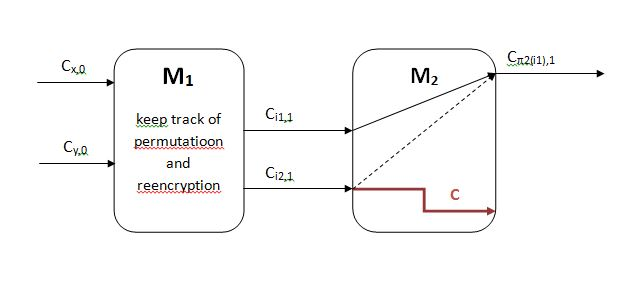
\includegraphics[scale=0.4]{rpc.jpg}
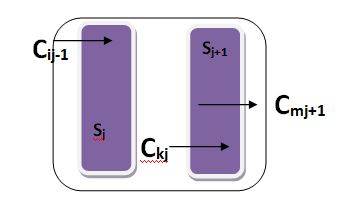
\includegraphics[scale=0.4]{duds.jpg} 
\end{center}

\framebreak

\begin{block}{Boundary Check}
\begin{itemize}
\item Let $k$ minimum number of votes to alter election result.
\item What is the probability $Pr_{und}$ that someone switches $k$ votes without detection; If $p=\frac{1}{2}n$ permutations are revealed then  $Pr_{und} = \frac{1}{2^k}$
\item Proof idea: 
\begin{itemize}
\item Since mix servers are paired, we check only predecessors or successors of intermediate items.
\item If a mix server is not honest, we will find it out by checking predessor or successor.
\item Testing is independent.
\end{itemize}
\end{itemize}
\end{block}

 
 

\end{frame}

\begin{frame}[allowframebreaks]{Almost Entirely Correct Mixing \cite{BG02}}

\begin{itemize}
\item \textbf{Idea}: We might not need a 100\% correct proof of mixing, especially if the margin of victory is wide.
\item An almost correct proof of mixing might do.
\item $10^6$ votes -> instant proof and 99\% correct proof of mixing.
\end{itemize}

\begin{block}{Method}
\begin{itemize}
\item Select a random subset $S$ of mix server inputs
\item Calculate the product $\pi_s$
\item Reveal $S$ to the mix server.
\item Ask to product a set of outputs $S'$ st. $\pi_s = \pi_{s'}$
\item Honest mix server:  Simply apply the permutation
\item Cheating mix server: Might be impossible to find such $S'$.
\end{itemize}
\end{block}

\begin{block}{Operation}
\begin{itemize}
\item  Input Ciphertexts $C_i = (g^{r_{i}},m_i \cdot y^{r_{i}})$
\item  Output Ciphertexts $C_{\pi(i)} = (g^{r'_{i}},m'_i \cdot y^{r'_{i}})$
\item Each server $M_j$ generates and commits to random $r_j$. $r = \oplus_j r_j$
\item Agree on a security parameter $\alpha$.
\item Verify correct format of output with a single exponentiation.
\item Each Mix-Server $M_j$ proves that $ \prod_{i=1}^n m_i =  \prod_{i=1}^n m'_i $ using El Gamal homomorphism and Chaum-Pedersen.
\item Generate $\alpha$ sets $S_1,\cdots,S_{\alpha}, S_i \subset S$ by including each input item with probability $\frac{1}{2}$ where randomness stems from r.
\end{itemize}
\end{block}


\begin{block}{Operation}
\begin{itemize}
\item The sets $S_1,\cdots,S_{\alpha}$ are given to $M_j$.
\item $M_j$ must produce $S'_1,\cdots,S'_{\alpha}$ st. $\forall i \in \{ 1,\cdots \alpha \} \|S_i\| = \|S'_i\|$ and 
$\prod_{k \in S_i}  m_i =  \prod_{k \in S'_i}  m'_i $. Proof is given using El Gamal homomorphism and Chaum-Pedersen.
\item If a server fails in the previous test it is considered dishonest and is excluded and the protocol is restarted.
\item If the protocol succeeds then the ballots are decrypted.
\end{itemize}
\end{block}

\begin{block}{Properties for $k$ mix servers and $n$ inputs}
\begin{itemize}
\item Proof Cost = $2\alpha(2k-1)$ exponentiations
\item Decryption Cost = $(2+4k)n$
\item Privacy Every input is hidden among $n/2^\alpha$.
\item Cheating will be detected with probability $1-\frac{5}{8}^{\alpha}$ or the DLOG problem can be solved in polynomial time.
\end{itemize}
\end{block}

\begin{block}{Example}
\begin{itemize}
\item Election with 160K voters
\item $\alpha = 6$ subsets to check per server
\item Every vote is hidden in 2500 votes
\item Cheating will be detected with probability $94\%$
\end{itemize}
\end{block}

\end{frame}

\begin{frame}[allowframebreaks]{Optimistic Mixing \cite{Opt02}}

\begin{itemize}
\item Exit - Poll Mixing
\item El Gamal Re encryption Mixnet
\item Fast proof when all mix servers are honest
\item If a cheating mix server is found then:
\begin{itemize}
	\item No output is produced
	\item A correct proof is executed (\cite{Neff01},\cite{FS01})
	\item Privacy is not compromised
\end{itemize}
\item Design to execute several mix sessions with the same set of keys
\item Proofs of knowledge are bound to a session id
\end{itemize}

\framebreak

{Proof of Product with checksum}
\begin{itemize}
\item Input: Encryption of Plaintexts with cryptographic checksum
\item Proof of Correct Operation: $ \prod_{input}plaintexts = \prod_{output}plaintexts $ without knowledge of the plaintexts (for privacy reasons)
\item Product Preservation does not imply absence of cheating
\item If cheating occurs some plaintexts will have been replaced so that the product is not altered
\item The checksums will still be invalid
\item \textbf{Cause:} Cheating Mix Server Or Invalid checksum in the first place?

\end{itemize}

\framebreak

\begin{block}{Solution}
\begin{itemize}
\item Restrict the input plaintexts $m_i$ (\textit{and} the output plaintexts $m'_i$) to a particular format so that it is infeasible
$ \{m_i\} \neq \{m'_i\} $ and $ \prod m_i = \prod m'_i $
\item \textbf{How:} Apply a hash function to the input.
\item $(E(m,r), E(h(m),r'))$
\item \textbf{Theorem (Wagner):}
It is impossible to find two different lists of ciphertexts of equal length $ \{(u_i,v_i)\}_{i=1}^N \neq \{(u'_i,v'_i)\}_{i=1}^N $ 
such that $ \prod_{i=1}^N h(u_i,v_i) = \prod_{i=1}^N h(u'_i,v'_i) $ in a group where the discrete logarithm is hard
\end{itemize}
\end{block}

\begin{block}{Privacy compromise}
\begin{itemize}
\item \textbf{Remark:}Cheating will be detected \textbf{after the fact}. Not much can be done if privacy has been compromised (there is no use in mixing again:
\item For example:
\begin{itemize}
\item User $i$ submits $t_i = ( \, E(m_i,r_i), E(h(m_i),r'_i) \, )$
\item Cheating mix server replaces $u_1$ with $ t_1 \cdot t_2$ and $t_2$ with $(1,1,1,1)$.
\item Cheating will be discovered after the decryption
\item The cheating server will be disqualified but
\item If mixing is restarted the cheating server will be able to distinguish the output of the first two users from the outputs of the rest by comparing the output of the second run with the output of the first run by checking for the product of the two plaintexts
\end{itemize}
\end{itemize}
\end{block}

\framebreak

\textbf{Solution:Double Enveloping}
\begin{itemize}
\item User input is encrypted twice
\item Each user submits the triple: $ t_i = ( \, E(G_i,r_i), E(M_i,r'_i), E(h(M,G),r''_i) \, )$  where $(G_i,M_i) = (g^{r_i},m \cdot y^{r_i}) = E(m_i,r_i)$
\item Verification Step: Decrypt Once
\item If verification succeeds (both product and checksum) then decrypt twice and tally
\item If cheating is discovered then encrypted inputs the cause of cheating is sought:
\begin{itemize}
\item Cheating senders: Solution: Ignore them, and proceed with the rest
\item Cheating mix servers: The messages will be forwarded to the slower mixnet with the mix server replaced
\end{itemize}
\item Cheating will not expose privacy, since the cheating server will cheat on (single) ciphertexts
\end{itemize}


\framebreak

\textbf{Investigation of Invalid Triples}
\begin{itemize}
\item Invalid triples $ w_i \neq h(u_i,v_i) $
\item Backtrace their path through the mixnet
\item Last server reveals: (input, randomisation)
\item Validate that the triple can be obtained from the input
\item Repeat until the first server
\item If the first server is reached then classify as user cheating
\item If a server fails validation the classify as server cheating
\end{itemize}


\end{frame}

\section{Conclusion}

\begin{frame}{Further Work:Review}
\begin{itemize}
\item Attacks
\item Voting based on Homomorphic Encryption
\item Voting based on Blind Signatures
\item Voter Verification Methods (visual cryptography)
\item Implementations (Helios, Scratch \& Vote, PretaVoter)
\end{itemize}
\end{frame}

\begin{frame}[allowframebreaks]{References}
\begin{small}
\bibliographystyle{alpha}
\bibliography{mixref}
\end{small}
\end{frame}

 
\end{document}
